\subsection{Explicación del algoritmo implementado}

Para resolver el problema de CMF utilizaremos el algoritmo de Bron-Kerbosch con algunas modificaciones. Dado un grafo G, el algoritmo de Bron-Kerbosch busca todas las cliques maximales de G utilizando una técnica de backtracking recursivo. Más generalmente, dados tres conjuntos R, P y X, R forma cliques recolectando nodos de P y X. P le brinda posibles nodos candidatos a R para armar cliques mientras que el conjunto X se encuentra conformado por vértices que ya fueron utilizados previamente para la extensión de la clique en R y que por lo tanto no se tienen en cuenta. Para cada nodo $v$ en P se hace una llamada recursiva en donde $v$ es agregado a R y, P y X se restringen a todos los nodos adyacentes a $v$. Luego, se mueve el nodo $v$ de P al conjunto X y se continúa con un nuevo vértice de P para formar nuevas cliques.

La recursión se inicia seteando a R y a X como conjuntos vacíos y a P como el conjunto conformado por todos los nodos del grafo. Por cada llamado recursivo, el algoritmo chequea si los conjuntos P y X se encuentran vacíos y, en caso de estarlos, reporta a R como clique maximal. Sin embargo, nuestro algoritmo no realiza el último paso descripto ya que el objetivo es encontrar la clique de máxima frontera. En vez de verificar si los conjuntos P y X están vacíos, calcula el cardinal de la frontera de la clique formada en R y en caso de ser mayor que la encontrada hasta ese momento de ejecución, la guarda. A continuación un pseudocódigo del algoritmo:

\begin{algorithm}[H]
\caption{findCliques}\label{ej1}
\begin{algorithmic}[1]
\Procedure{findCliques}{$R,P,X$}
	\State int $front$ $\shortleftarrow$ frontera(R)
	\If {front $>$ maxFrontera}
		\State cliqueMaxFrontera $\shortleftarrow$ R
		\State maxFrontera $\shortleftarrow$ front
	\EndIf
	\ForAll{$p\ vertice \in\ P$}
		\State findCliques(R $\cup$ $\{v\}$, P $\cap$ N(v), X $\cap$ N(v))
	\EndFor
\EndProcedure
\end{algorithmic}
\end{algorithm}

Algunas aclaraciones:
\begin{itemize}
	\item N(v) es el conjunto de todos los nodos adyacentes a $v$ en el grafo.
	\item frontera(R) calcula el cardinal de la frontera de la clique R.
	\item $cliqueMaxFrontera$ guarda los nodos de la clique de máxima frontera y $maxFrontera$ almacena el cardinal de la frontera de dicha clique.
\end{itemize}

\subsubsection{Ejemplo de ejecución}

\begin{figure}[H]
 \centering
  \subfloat[]{
   \label{}
    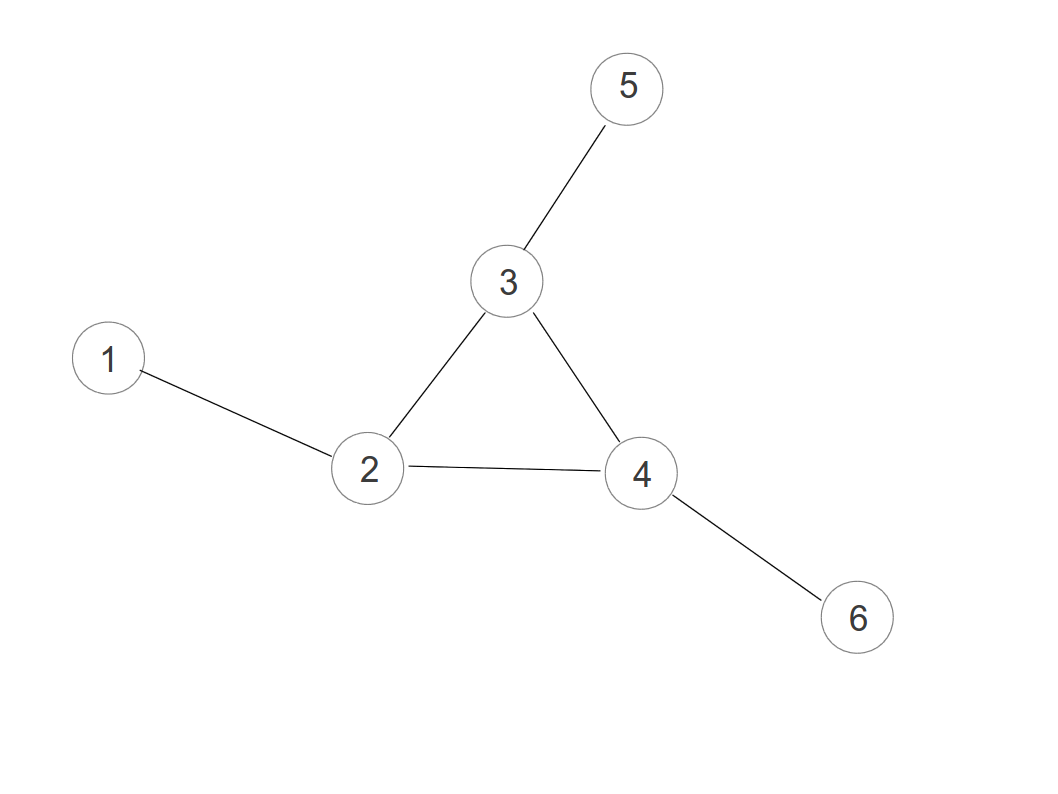
\includegraphics[scale=0.3]{exacto/imgs/ejemplito.png}}
  \subfloat[Frontera=4.]{
   \label{}
    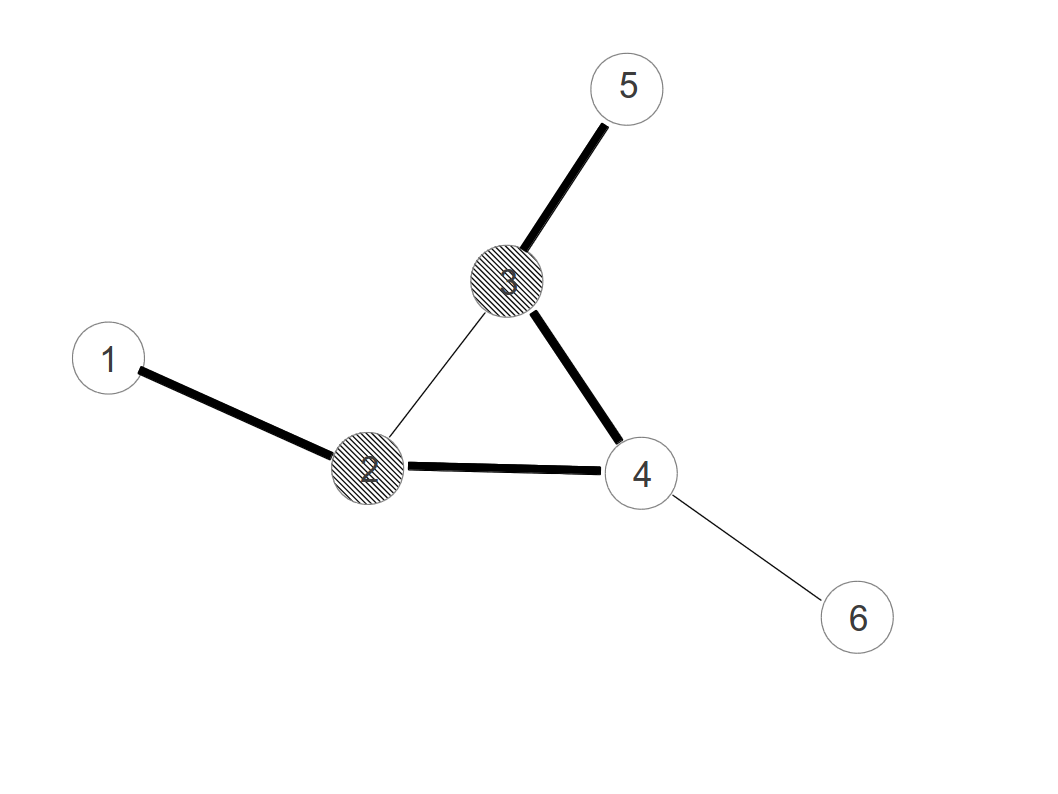
\includegraphics[scale=0.3]{exacto/imgs/ejemplitoSol.png}}
\caption{Un ejemplo y su solución}

\end{figure}

\begin{center}
    \begin{tabular}{ | l | l | l | l | l | p{5cm} |}
    \hline
    Llamada recursiva & R & P & X & cliqueMaxFrontera & Comentarios \\ \hline
    1 & $\{$ $\}$ & $\{$1,2,3,4,5,6$\}$ & $\{$ $\}$ & $\{$ $\}$ & Candidatos: todos los nodos del grafo. \\ \hline
    2 & $\{$1$\}$ & $\{$2$\}$ & $\{$ $\}$ & $\{$1$\}$ Frontera: 1 & Formo la clique R y el único candidato posible es el nodo 2 (único adyacente).\\ \hline
    3 & $\{$1,2$\}$ & $\{$ $\}$ & $\{$ $\}$ & $\{$1,2$\}$ Frontera: 2 & La clique R no puede agregar más nodos. Los adyacentes a 2 no son adyacentes a 1. \\ \hline
    4 & $\{$2$\}$ & $\{$3,4$\}$ & $\{$1$\}$ & $\{$2$\}$ Frontera: 3 & La clique R tiene dos candidatos para agregar (sus adyacentes) pero no puede agregar el nodo 1 que se encuentra en X ya que esa clique ya fue analizada previamente.\\ \hline
    5 & $\{$2,3$\}$ & $\{$4$\}$ & $\{$ $\}$ & $\{$2,3$\}$ Frontera: 4 & Candidato: 4. Adyacente a 2 y 3.\\ \hline
    6 & $\{$2,3,4$\}$ & $\{$ $\}$ & $\{$ $\}$ & $\{$2,3$\}$ Frontera: 4  &\\ \hline
    7 & $\{$2,4$\}$ & $\{$ $\}$ & $\{$ $\}$ & $\{$2,3$\}$ Frontera: 4 & El 3 no es candidato ya que fue evaluada esa opción previamente. \\ \hline
    8 & $\{$3$\}$ & $\{$4,5$\}$ & $\{$ $\}$ & $\{$2,3$\}$ Frontera: 4 & El 2 no es candidato ya que fue evaluada esa opción previamente.\\ \hline
    9 & $\{$3,4$\}$ & $\{$ $\}$ & $\{$ $\}$ & $\{$2,3$\}$ Frontera: 4 & \\ \hline
    10 & $\{$3,5$\}$ & $\{$ $\}$ & $\{$ $\}$ & $\{$2,3$\}$ Frontera: 4 & \\ \hline
    11 & $\{$4$\}$ & $\{$6$\}$ & $\{$ $\}$ & $\{$2,3$\}$ Frontera: 4 & \\ \hline
    12 & $\{$4,6$\}$ & $\{$ $\}$ & $\{$ $\}$ & $\{$2,3$\}$ Frontera: 4 & \\ \hline
    13 & $\{$5$\}$ & $\{$ $\}$ & $\{$ $\}$ & $\{$2,3$\}$ Frontera: 4 & \\ \hline
    14 & $\{$6 $\}$ & $\{$ $\}$ & $\{$ $\}$ & $\{$2,3$\}$ Frontera: 4 & \\
	\hline
    \end{tabular}
\captionof{table}{Seguimiento del algoritmo. Solución devuelta: $\{$2,3$\}$, frontera: 4.}
\end{center}

